\documentclass[11pt,a4paper]{article}
\usepackage[utf8]{inputenc}
\usepackage{amsmath}
\usepackage{amsfonts}
\usepackage{amssymb}
\usepackage{makeidx}
\usepackage{graphicx}
\usepackage{lmodern}
\usepackage{kpfonts}
\usepackage{xcolor}
\usepackage{cancel}
\usepackage{mathtools}
\usepackage{schemata}
\usepackage{cancel}
\providecommand{\abs}[1]{\lvert#1\rvert}%Sirve para colocar valores absolutos
\providecommand{\norm}[1]{\lVert#1\rVert}%Sirve para colocar módulo
\usepackage[left=2.00cm, right=2.00cm, top=2.00cm,bottom=2.00cm]{geometry}
\author{Harold Alessander Jhon Zambrano Quispe}
\title{SOLUCIONARIO DE LA TAREA 1}
\begin{document}
   \begin{titlepage}%Habilita una pagina sin enumerar.
	\begin{center}
	 {\huge \textbf{Universidad Nacional de Ingeniería}}\\
	 \vspace{3mm}
	  {\Large {Facultad de Ingeniería Eléctrica y Electrónica}}\\
	\vspace{-5mm}	 
	 \begin{figure}[h]
	 	\centering 
	 	
\includegraphics[scale=0.5]{Logo UNI}
	 \end{figure}
	 \vspace{-6mm}
	{\Large {Especialidad de Ingeniería de Telecomunicaciones}}\\
	\vspace{3mm}
	{\Large \textbf{"Laboratorio 1 de Análisis de Señales y Sistemas"}}\\
	\vspace{8mm}
	\begin{flushleft}
	{\Large {\textbf{Curso}: Análisis de Señales y Sistemas}}\\
	\vspace{8mm}		
	{\Large {\textbf{Código del Curso}: EE410-M}}\\	
	\vspace{8mm}	
	{\Large {\textbf{Docente}: Manuel Arevalo Villanueva}}\\
	\vspace{8mm}	
	{\Large {\textbf{Integrantes}: 
	Gian Carlos Chancavilcas Osores - 20191108K\\
	\vspace{4mm}
	\hspace{3cm}Julio Cesar Luna Yabarrena - 20130346I\\ 
	\vspace{4mm}
	\hspace{3cm}Harold Alessander Jhon Zambrano Quispe - 20191351B}}\\
	\vspace{8mm}	
	\end{flushleft}
	\vspace{10mm}
	{\Huge {\textbf{2021-I}}}\\
	\end{center}
\end{titlepage}
%Se debe compilar desde la funcion principal
   \section{{INTRODUCCIÓN}}{
	\large{
	hOLA

	}}
	\newpage
   \section{{MARCO TEÓRICO}}{
	\large{
	\begin{enumerate}
	\item[\textbf{3)}]
	\begin{flushleft}
\textbf{CONVOLUCI\'ON DISCRETA:}
\end{flushleft}
Convolución es un valor que se extiende a todos los sistemas que son invariantes linear del tiempo (LTI - Linear Time Invariant). La idea de convolución discreta es la misma que la de convolución continua. Por esta razón, puede ser de gran ayuda el ver las dos versiones para que usted entienda la extrema importancia del concepto. Recuerde que la convolución es un instrumento poderoso al determinar el resultado de un sistema después de saber la una entrada arbitraria y la respuesta al impulso del sistema. 
\begin{flushleft}
\textbf{SUMA DE CONVOLUCIÓN}
\end{flushleft}
Como ya ha sido mencionado, la suma de convolución provee una manera matemáticamante concisa para expresar el resultado de un sistema LTI, basado en una entrada arbitraria para una señal discreta y también el saber la respuesta del sistema. La suma de convolución es expresada como:
$$\boxed{y[n]=x[n]*h[n]=\sum_{k=-\infty}^{\infty}x[k]h[n-k]}$$
	\end{enumerate}
	}}
\newpage
	\section{{\large \textbf{2. Sea $f[n]=3$ , $0\leq n \leq 2$, un pulso cuadrado , $g[n]=[1,2,3,2,1]$ un pulso triangular , sea $h[n]=(\frac{1}{2})^n$ , $0\leq n\leq 8$ una amortiguación exponencial}}}{
	\large{
	\begin{enumerate}
	\item[\textbf{a)}]
	\textbf{Usando el MATLAB grafique las señales en tiempo discreto f[n],g[n] y h[n].}\\
	$ \bullet$Para la grafica $f[n]=3$ , $ 0\leq n\leq 2$, se utilizo la funcion stem de MATLAB para realizar un pulso cuadrado consideramos en un intervalo de $[-8,8]$.
\begin{figure}[h]
\centering
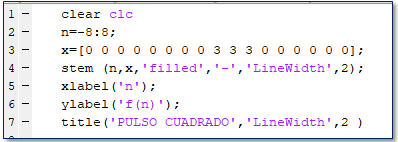
\includegraphics[scale=0.6]{../Imagenes de señales problema 2/Sin título.png} 
\end{figure}

\begin{figure}[h]
\centering
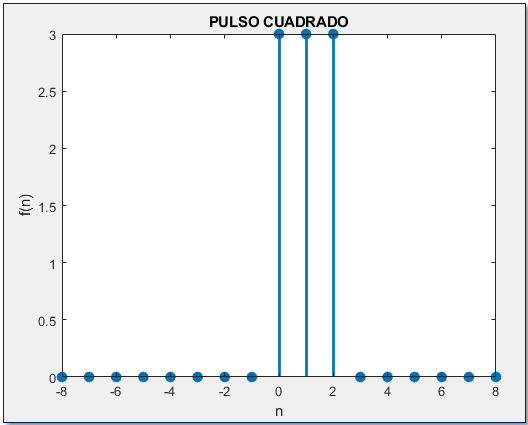
\includegraphics[scale=0.5]{../Imagenes de señales problema 2/pulso.png} 
\caption{Código en Matlab y gráfica de f[n]} 
\label{Gráfica_fn}
\end{figure}
$\bullet$Para la gráfica $g[n]=[1,2,3,2,1]$ , $-2\leq n\leq 2$, se utilizo la función stem de MATLAB para realizar un pulso rectangular consideramos en un intervalo de $[-8,8]$.

\begin{center}
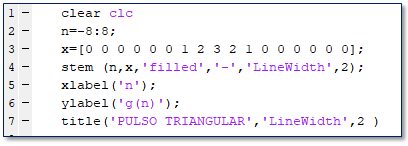
\includegraphics[scale=0.6]{../Imagenes de señales problema 2/sintutulo1.png}
\end{center}

\begin{figure}[h]
\centering
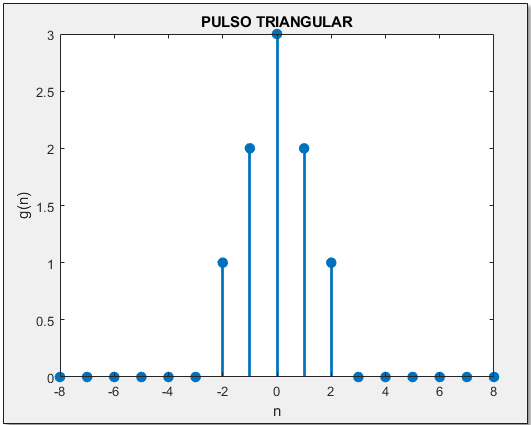
\includegraphics[scale=0.5]{../Imagenes de señales problema 2/triangulo.png} 
\caption{Código en Matlab y gráfica de g[n]} 
\label{Gráfica_gn}
\end{figure}
\newpage
$\bullet$Para la grafica $h[n]=(\frac{1}{2})^n$, se utilizo la funcion stem de MATLAB para realizar la amortiguación exponencial $[-8,8]$ con paso 1.
\begin{figure}[h]
\centering
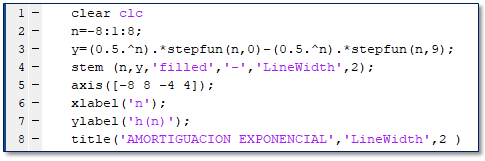
\includegraphics[scale=0.6]{../Imagenes de señales problema 2/titulo2.png} 
\label{Código_hn}
\end{figure}

\begin{figure}[h]
\centering
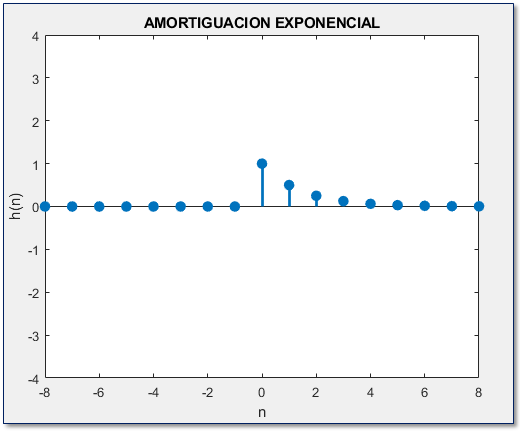
\includegraphics[scale=0.6]{../Imagenes de señales problema 2/expone.png} 
\caption{Código en Matlab y gráfica de h[n]}
\label{Gráfica_hn}
\end{figure}
	\item[\textbf{b)}]
	\textbf{Encuentre en términos de n y la señal escalón unitario las siguientes convoluciones:}\\
Como nos piden la convolución de dos señales discretas por conocimiento previo:
$$\boxed{y[n]=x[n]*h[n]=\sum_{k=-\infty}^{\infty}x[k]h[n-k]}$$
$\bullet$ Hallamos la convolución de $f[n]*g[n]$ con la formula previa hallada.
$$n<-2 \rightarrow y[n]=0$$
$$n=-2 \rightarrow y[n]=\sum_{k=-\infty}^{\infty}f[k]g[n-k]=f[0]g[-2]=(3)(1)=3$$
$$n=-1 \rightarrow y[n]=\sum_{k=-\infty}^{\infty}f[k]g[n-k]=f[0]g[-1]+f[1]g[-2]=9$$
$$n=0 \rightarrow y[n]=\sum_{k=-\infty}^{\infty}f[k]g[n-k]=f[0]g[n]+f[1]g[-1]+f[2]g[-2]=18$$
$$n=1 \rightarrow y[n]=\sum_{k=-\infty}^{\infty}f[k]g[n-k]=f[0]g[1]+f[1]g[0]+f[2]g[-1]=21$$
$$n=2 \rightarrow y[n]=\sum_{k=-\infty}^{\infty}f[k]g[n-k]=f[0]g[2]+f[1]g[1]+f[2]g[0]=18$$
$$n=3 \rightarrow y[n]=\sum_{k=-\infty}^{\infty}f[k]g[n-k]=f[1]g[2]+f[2]g[1]=9$$\\
$$n=4 \rightarrow y[n]=\sum_{k=-\infty}^{\infty}f[k]g[n-k]=f[2]g[2]=3$$\\
$$n>4 \rightarrow y[n]=0$$
\begin{equation*}
y[n]=f[n]*g[n] =
\begin{cases}
0 & \text{si $n<-2 $}\\
3 & \text{si $n= -2$}\\
9 & \text{si $n= -1$}\\
18 & \text{si $n= 0$}\\
21 & \text{si $n= 1$}\\
18 & \text{si $n= 2$}\\
9 & \text{si $n= 3$}\\
3 & \text{si $n=4$}\\
0 & \text{si $n>4$}
\end{cases}
\end{equation*}\\
\textbf{Expresamos en n y escalón unitario la señal:}
$$\boxed{y[n]=3u[n+2]+6u[n+1]+9u[n]+3u[n-1]-3u[n-2]-9u[n-3]-6u[n-4]-3u[n-5]}$$

$\bullet$ Hallamos la convolución de $f[n]*h[n]$ con la formula previa hallada.
$$f[n]*h[n]=\sum_{k=-\infty}^{\infty}f[k]h[n-k]$$
$$n<0 \rightarrow y[n]=0$$
$$n=0 \rightarrow y[n]=\sum_{k=-\infty}^{\infty}f[k]h[n-k]=f[0]h[0]=3$$
$$n=1 \rightarrow y[n]=\sum_{k=-\infty}^{\infty}f[k]h[n-k]=f[0]h[1]+f[1]h[0]=\frac{9}{2}$$
$$n=2 \rightarrow y[n]=\sum_{k=-\infty}^{\infty}f[k]h[n-k]=f[0]h[2]+f[1]h[1]+f[2]h[0]=\frac{21}{4}$$
$$n=3 \rightarrow y[n]=\sum_{k=-\infty}^{\infty}f[k]h[n-k]=f[0]h[3]+f[1]h[2]+f[2]h[1]=\frac{21}{8}$$
$$n=4 \rightarrow y[n]=\sum_{k=-\infty}^{\infty}f[k]h[n-k]=f[0]h[4]+f[1]h[3]+f[2]h[2]=\frac{21}{16}$$
$$n=5 \rightarrow y[n]=\sum_{k=-\infty}^{\infty}f[k]h[n-k]=f[0]h[5]+f[1]h[4]+f[2]h[3]=\frac{21}{32}$$
$$n=6 \rightarrow y[n]=\sum_{k=-\infty}^{\infty}f[k]h[n-k]=f[0]h[6]+f[1]h[5]+f[2]h[4]=\frac{21}{64}$$
$$n=7 \rightarrow y[n]=\sum_{k=-\infty}^{\infty}f[k]h[n-k]=f[0]h[7]+f[1]h[6]+f[2]h[5]=\frac{21}{128}$$
$$n=8 \rightarrow y[n]=\sum_{k=-\infty}^{\infty}f[k]h[n-k]=f[0]h[8]+f[1]h[7]+f[2]h[6]=\frac{21}{256}$$
$$n=9 \rightarrow y[n]=\sum_{k=-\infty}^{\infty}f[k]h[n-k]=f[1]h[8]+f[2]h[7]=\frac{9}{256}$$
$$n=10 \rightarrow y[n]=\sum_{k=-\infty}^{\infty}f[k]h[n-k]=f[2]h[8]=\frac{3}{256}$$
$$n>10 \rightarrow y[n]=\sum_{k=-\infty}^{\infty}f[k]h[n-k]=0$$
\begin{equation*}
y[n]=f[n]*h[n] =
\begin{cases}
0 & \text{si $n<0 $}\\
3 & \text{si $n= 0$}\\
\frac{9}{2} & \text{si $n= 1$}\\
\frac{21}{4} & \text{si $n= 2$}\\
\frac{21}{8} & \text{si $n= 3$}\\
\frac{21}{16} & \text{si $n= 4$}\\
\frac{21}{32} & \text{si $n= 5$}\\
\frac{21}{64} & \text{si $n=6$}\\
\frac{21}{128} & \text{si $n=7$}\\
\frac{21}{256} & \text{si $n=8$}\\
\frac{9}{256} & \text{si $n=9$}\\
\frac{3}{256} & \text{si $n=10$}\\
0 & \text{si $n>10$}
\end{cases}
\end{equation*}\\
\textbf{Expresamos en n y escalón unitario la señal:}
$$\boxed{y[n]=(0.5)^n(3u[n]+6u[n-1]+12u[n-2]-12u[n-9])-(0.5)^8(6u[n-10]-3u[n-11])}$$
$\bullet$ Hallamos la convolución de $g[n]*h[n]$ con la formula previa hallada.
$$g[n]*h[n]=\sum_{k=-\infty}^{\infty}g[k]h[n-k]$$
$$n<-2 \rightarrow y[n]=0 $$
$$n=-2 \rightarrow y[n]=\sum_{k=-\infty}^{\infty}g[k]h[n-k]=g[-2]h[0]=1 $$
$$n=-1 \rightarrow y[n]= \sum_{k=-\infty}^{\infty}g[k]h[n-k]=g[-1]h[0]+g[-2]h[1]=\frac{5}{2} $$
$$n=0 \rightarrow y[n]= \sum_{k=-\infty}^{\infty}g[k]h[n-k]=g[-2]h[2]+g[-1]h[1]+g[0]h[0]=\frac{17}{4} $$
$$n=1 \rightarrow y[n]= \sum_{k=-\infty}^{\infty}g[k]h[n-k]=g[-2]h[3]+g[-1]h[2]+g[0]h[1]+g[1]h[0]=\frac{33}{8} $$
$$n=2 \rightarrow y[n]= \sum_{k=-\infty}^{\infty}g[k]h[n-k]=g[-2]h[4]+g[-1]h[3]+g[0]h[2]+g[1]h[1]+g[2]h[0]=\frac{49}{16} $$
$$n=3 \rightarrow y[n]= \sum_{k=-\infty}^{\infty}g[k]h[n-k]=g[-2]h[5]+g[-1]h[4]+g[0]h[3]+g[1]h[2]+g[2]h[1] =\frac{49}{32}$$
$$n=4 \rightarrow y[n]= \sum_{k=-\infty}^{\infty}g[k]h[n-k]=g[-2]h[6]+g[-1]h[5]+g[0]h[4]+g[1]h[3]+g[2]h[2]=\frac{49}{64} $$
$$n=5 \rightarrow y[n]= \sum_{k=-\infty}^{\infty}g[k]h[n-k]=g[-2]h[7]+g[-1]h[6]+g[0]h[5]+g[1]h[4]+g[2]h[3]=\frac{49}{128} $$
$$n=6 \rightarrow y[n]= \sum_{k=-\infty}^{\infty}g[k]h[n-k]=g[-2]h[8]+g[-1]h[7]+g[0]h[6]+g[1]h[5]+g[2]h[4]=\frac{49}{256} $$
$$n=7 \rightarrow y[n]= \sum_{k=-\infty}^{\infty}g[k]h[n-k]=g[-1]h[8]+g[0]h[7]+g[1]h[6]+g[2]h[5]=\frac{3}{32} $$
$$n=8 \rightarrow y[n]= \sum_{k=-\infty}^{\infty}g[k]h[n-k]=g[0]h[8]+g[1]h[7]+g[2]h[6] =\frac{11}{256}$$
$$n=9 \rightarrow y[n]= \sum_{k=-\infty}^{\infty}g[k]h[n-k]=g[1]h[8]+g[2]h[7]=\frac{1}{64} $$
$$n=10 \rightarrow y[n]= \sum_{k=-\infty}^{\infty}g[k]h[n-k]=g[2]h[8]=\frac{1}{256}$$
$$n>10 \rightarrow y[n]=0 $$
\begin{equation*}
y[n]=g[n]*h[n] =
\begin{cases}
0 & \text{si $n<-2 $}\\
1 & \text{si $n= -2$}\\
\frac{5}{2} & \text{si $n= -1$}\\
\frac{17}{4} & \text{si $n= 0$}\\
\frac{33}{8} & \text{si $n= 1$}\\
\frac{49}{16} & \text{si $n= 2$}\\
\frac{49}{32} & \text{si $n= 3$}\\
\frac{49}{64} & \text{si $n=4$}\\
\frac{49}{128} & \text{si $n=5$}\\
\frac{49}{256} & \text{si $n=6$}\\
\frac{3}{32} & \text{si $n=7$}\\
\frac{11}{256} & \text{si $n=8$}\\
\frac{1}{64} & \text{si $n=9$}\\
\frac{1}{256} & \text{si $n=10$}\\
0 & \text{si $n>10$}
\end{cases}
\end{equation*}\\
\textbf{Expresamos en n y escalón unitario la señal:}
$$y[n]=(0.5)^n(u[n+2]+4u[n+1]+12u[n]+16u[n-1]+16u[n-2]-49u[n-7])$$ $$+(0.5)^5(3u[n-7]-3u[n-8])
+(0.5)^8(11u[n-8]-11u[n-9])$$ $$+(0.5)^6(u[n-9]-u[n-10])+(0.5)^8(u[n-10]-u[n-11])$$
	\item[\textbf{c)}]	
	\textbf{Usando el comando conv en MATLAB grafique las convoluciones $$f[n]*f[n],f[n]*g[n],f[n]*h[n],g[n]*g[n], g[n]*h[n],h[n]*h[n]$$}
\textbf{Graficando}\\
 Como el algoritmo es igual para todos, solo bosquejamos las gráficas: 
\begin{center}
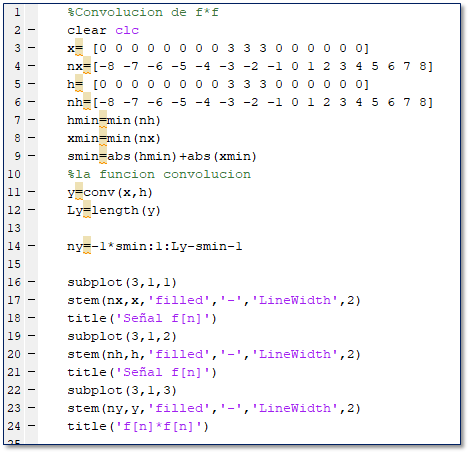
\includegraphics[scale=0.70]{../Imagenes de señales problema 2/ff.png} 
\end{center}
$$Convolucion :f[n]*f[n]$$ 
\begin{center}
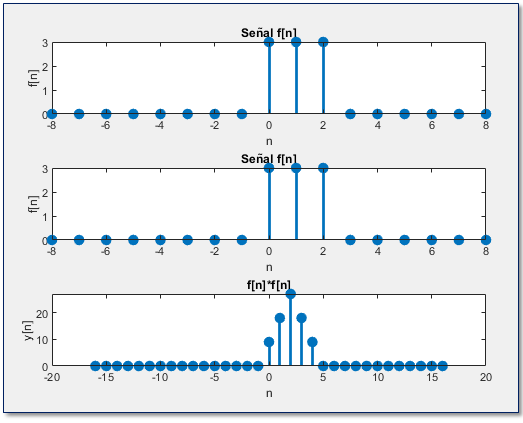
\includegraphics[scale=0.80]{../Imagenes de señales problema 2/ffgrafica.png} 
\end{center}
\newpage
$$Convolucion :f[n]*g[n]$$
\begin{center}
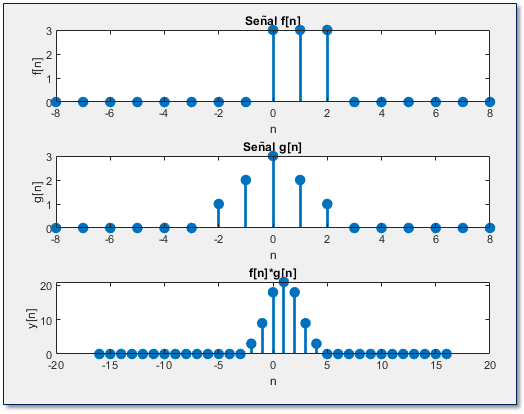
\includegraphics[scale=0.80]{../Imagenes de señales problema 2/fggrafica.png} 
\end{center}
$$Convolucion :f[n]*h[n]$$
\begin{center}
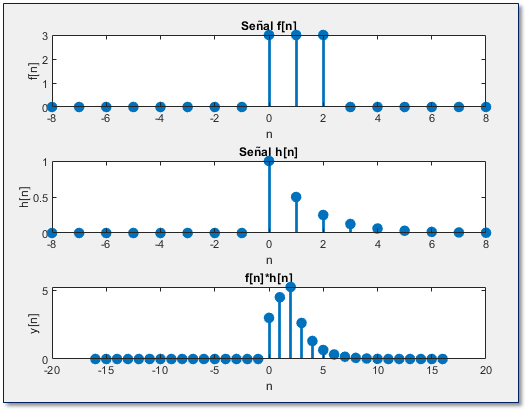
\includegraphics[scale=0.80]{../Imagenes de señales problema 2/fh.png} 
\end{center}
\newpage
$$Convolucion :g[n]*g[n]$$
\begin{center}
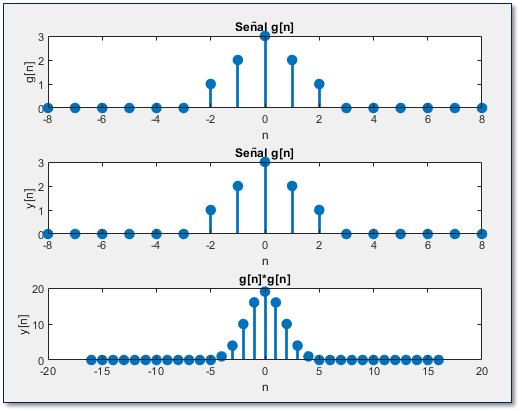
\includegraphics[scale=0.80]{../Imagenes de señales problema 2/gg.png} 
\end{center}
$$Convolucion :g[n]*h[n]$$
\begin{center}
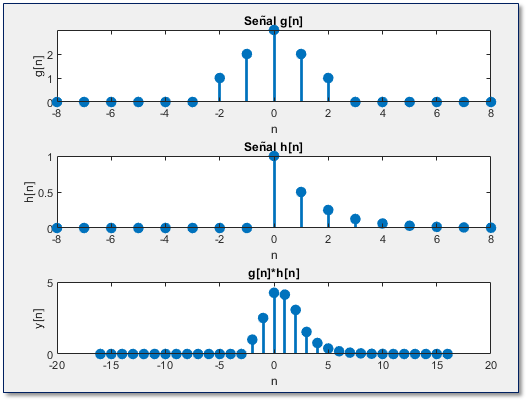
\includegraphics[scale=0.80]{../Imagenes de señales problema 2/gh.png} 
\end{center}
\newpage
$$Convolucion :h[n]*h[n]$$
\begin{center}
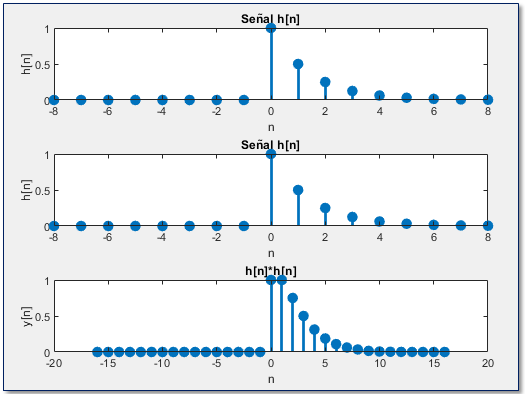
\includegraphics[scale=0.8]{../Imagenes de señales problema 2/hh.png} 
\end{center}
	\end{enumerate}
	}}
	\newpage
	\section{{\large 4.Considere un sistema causal LTI cuya entrada X(t) y salida Y(t) satisfacen $$Y^{''}(t)+2Y^{'}(t)+Y(t)=2X^{'}(t)+X(t)$$}}{
	\large{
	\begin{enumerate}
	\item[\textbf{a)}]
	\textbf{Usando la Transformada de Laplace encuentre un diagrama de bloques para dichos sistema. Usando el Simulink y el diagrama de bloques encuentre la respuesta del sistema al impulso $X_{1}[n]=\delta(t)$ , al escalón unitario $X_{2}(t)=u[n]$ , y a la amortiguación $X_{3}(t)=exp(-2t)$.}\\\\
	\textbf{Solución:}\\
	\textbf{$\bullet$ Realizando el diagrama de bloques del sistema causal LTI }\\\\
	\textbf{1er paso:} Calculando la función de transferencia del sistema.
	$$Y^{''}(t)+2Y^{'}(t)+Y(t)=2X^{'}(t)+X(t)$$
Aplicando la transformada de Laplace
%Simbolo para la transformada  de Laplace(\mathcal{L})
	\begin{eqnarray}
	\label{TransLaplaceDelSistema}
		\mathcal{L}{\lbrace Y^{''}(t)\rbrace}+2 \mathcal{L}{ \lbrace Y^{'}(t)\rbrace}+ \mathcal{L}{ \lbrace Y(t)\rbrace }=2 \mathcal{L}{\lbrace X^{'}(t)\rbrace}+ \mathcal{L}{ \lbrace X(t) \rbrace}
	\end{eqnarray}
	\textbf{Importante:} Transformada de Laplace que aplicaremos en (\ref{TransLaplaceDelSistema})\\ 
	$$\mathcal{L}{\lbrace Y^{''}(t)\rbrace}=s^2f(s)-sF(0)-F^{'}(0)$$
	$$\mathcal{L}{ \lbrace Y^{'}(t)\rbrace}=sf(s)-F(0)$$
	Para este sistema causal LTI, consideraremos que $F(0)=0$ y $F^{'}(0)=0$; por lo tanto, obtendremos lo siguiente:
	\begin{eqnarray}
	\label{TransLaplaceDe2Derivada}
		\mathcal{L}{\lbrace Y^{''}(t)\rbrace}=s^2f(s)
	\end{eqnarray}
	\begin{eqnarray}
	\label{TransLaplaceDe1Derivada}
		\mathcal{L}{ \lbrace Y^{'}(t)\rbrace}=sf(s)
	\end{eqnarray}
	Aplicando la transfomadas de Laplace (\ref{TransLaplaceDe1Derivada})
y (\ref{TransLaplaceDe2Derivada}) en la EDO (\ref{TransLaplaceDelSistema})
	$$s^2y(s)+2sy(s)+y(s)=2sx(s)+x(s)$$
	$$y(s)+ \dfrac{2y(s)}{s}+ \dfrac{y(s)}{s^2}= \dfrac{2x(s)}{s}+ \dfrac{x(s)}{s^2}$$
	\begin{eqnarray}
	\label{SistemaParaDBloque}
		y(s)= \dfrac{2x(s)}{s}+ \dfrac{x(s)}{s^2}- \dfrac{2y(s)}{s}- \dfrac{y(s)}{s^2}
	\end{eqnarray}
	\begin{eqnarray}
	\label{Función transferencia4}
	\boxed{h(s)=\dfrac{y(s)}{x(s)}=\dfrac{2s+1}{s^2 +2s+1}}
	\end{eqnarray}
	\newpage
\textbf{2do paso:}\\
Realizando el diagrama de bloques del sistema en Simulink, a partir de la ecuación (\ref{SistemaParaDBloque})
	
	\begin{figure}[h]
	\centering
	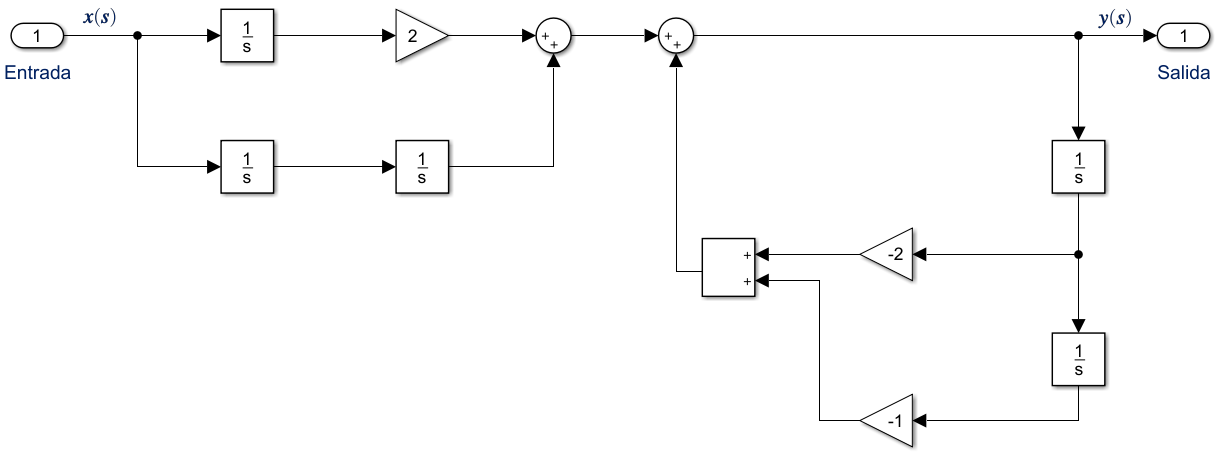
\includegraphics[scale=0.49]
{DIAGRAMABLOQUESISTEMA4} 
	\caption{Diagrama de bloque del sistema causal LTI}
\label{DIAGRAMABLOQUESISTEMA4}
\end{figure}
	
	Verificando si nuestro diagrama de bloque es correcta.
	\begin{figure}[h]
	\centering
	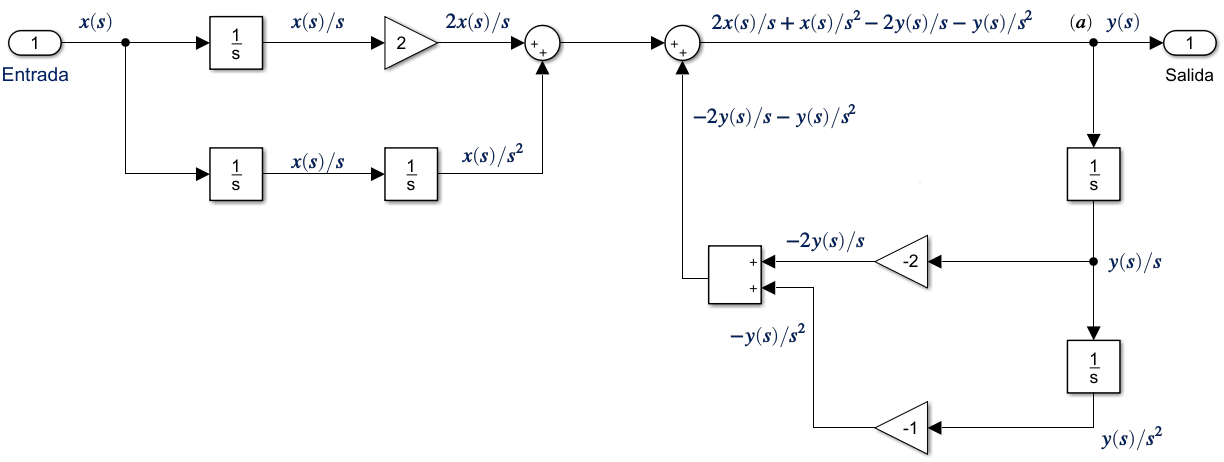
\includegraphics[scale=0.49]
{DIAGRAMABLOQUESISTEMA4VERIFICACION} 
	\caption{Verificacióndel diagrama de bloque del sistema causal LTI}
\label{DIAGRAMABLOQUESISTEMA4VERIFICACION}
\end{figure}
	Del diagrama de bloques de la figura (\ref{DIAGRAMABLOQUESISTEMA4VERIFICACION})
en (a), se verifica la ecuación (\ref{SistemaParaDBloque})\\
	$$y(s)= \dfrac{2x(s)}{s}+ \dfrac{x(s)}{s^2}- \dfrac{2y(s)}{s}- \dfrac{y(s)}{s^2}$$
	\newpage
 	$\bullet$ \textbf{Respuesta al impulso($X_1(t)=\delta (t))$}\\
	
	\begin{figure}[h]
	\centering
	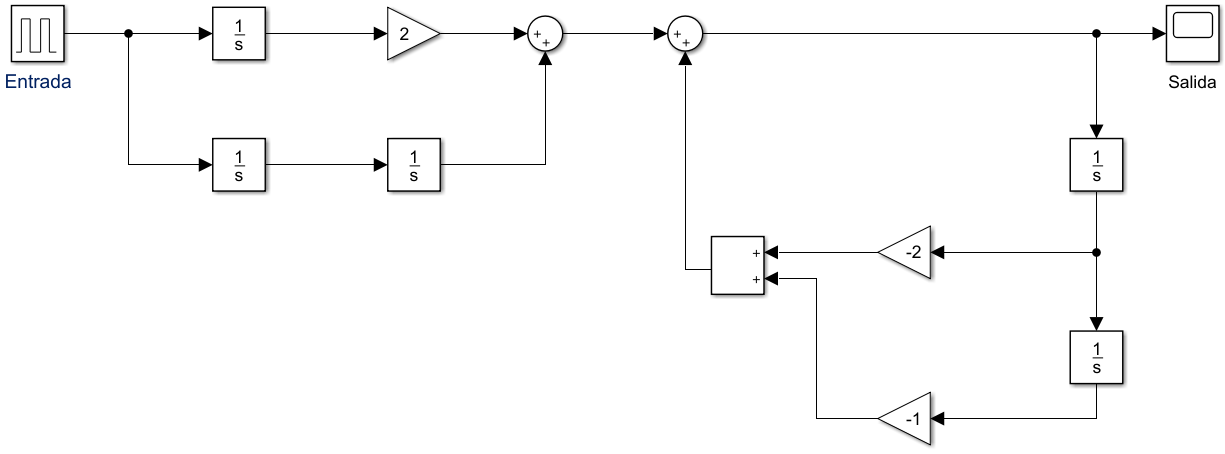
\includegraphics[scale=0.49]
{DIAGRAMADEIMPULSO} 
	\caption{Diagrama de bloques con entrada de un impulso}
\label{DIAGRAMADEIMPULSO}
\end{figure}
\begin{figure}[h]
	\centering
	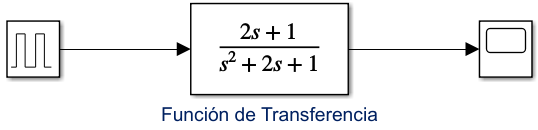
\includegraphics[scale=0.6]
{DIAGRAMADEIMPULSO2} 
	\caption{Otro diagrama de bloques con entrada de un impulso}
\label{DIAGRAMADEIMPULSO2}
\end{figure}
	Se puede verificar que en ambos diagramas de bloques se obtiene como respuesta, la siguiente respuesta con respecto al tiempo.
	\begin{figure}[h]
	\centering
	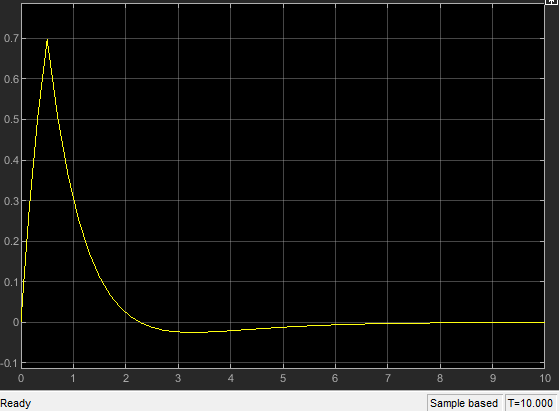
\includegraphics[scale=0.7]
{RESPUESTADELIMPULSO} 
	\caption{Otro diagrama de bloques con entrada de un impulso}
\label{RESPUESTADELIMPULSO}
\end{figure}
	\newpage
	
	$\bullet$ \textbf{Respuesta al escalón($X_2(t)= u(t))$}\\
	
	\begin{figure}[h]
	\centering
	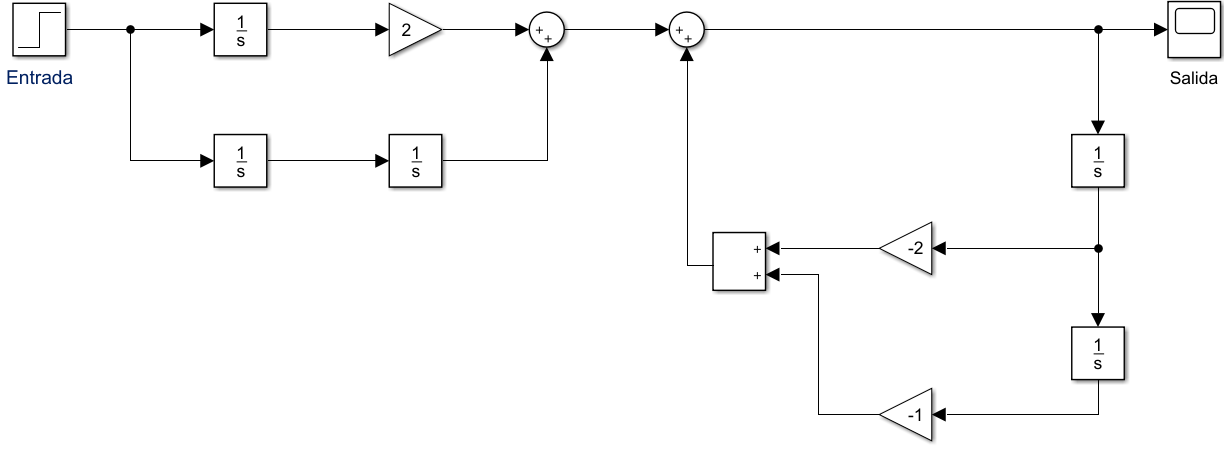
\includegraphics[scale=0.49]
{DIAGRAMADEESCALON} 
	\caption{Diagrama de bloques con entrada de un escalón}
\label{DIAGRAMADEESCALON}
\end{figure}
\begin{figure}[h]
	\centering
	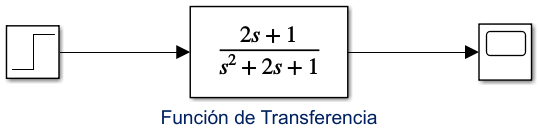
\includegraphics[scale=0.6]
{DIAGRAMADEESCALON2} 
	\caption{Otro diagrama de bloques con entrada de un escalón}
\label{DIAGRAMADEESCALON2}
\end{figure}
	Se puede verificar que en ambos diagramas de bloques se obtiene como respuesta, la siguiente respuesta con respecto al tiempo.
	\begin{figure}[h]
	\centering
	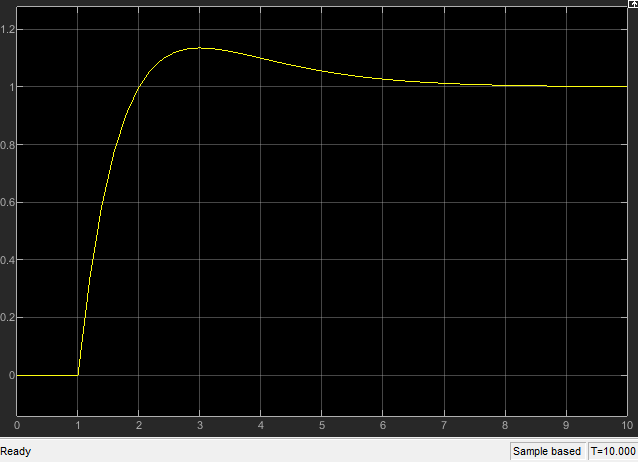
\includegraphics[scale=0.6]
{RESPUESTADELESCALON} 
	\caption{Otro diagrama de bloques con entrada de un escalón}
\label{RESPUESTADELESCALON}
\end{figure}
	\newpage
	
	\item[\textbf{b)}]
	\textbf{Encuentre las respuestas de la parte (a)en términos de t}\\\\
	$\bullet$\textbf{Respuesta al impulso($X_1(t)=\delta (t))$}\\
	$$y_1(s)=\mathcal{L}{\lbrace \delta (t) \rbrace}=1$$
	A partir de la función de transferencia(\ref{Función transferencia4})aplicaremos lo anterior.
	$$\dfrac{y_1(s)}{x_1(s)}=\dfrac{2s+1}{s^2 +2s+1}$$
	$$\dfrac{y_1(s)}{1}=\dfrac{2}{s+1}-\dfrac{1}{(s+1)^2}$$
	Aplicando transformada inversa de Laplace
	$$\dfrac{\mathcal{L^{-}}{\lbrace y_1(s)\rbrace }}{1}=2 \mathcal{L^{-}}{\lbrace \dfrac{1}{s+1} \rbrace } -\mathcal{L^{-}}{\lbrace \dfrac{1}{(s+1)^2}\rbrace}$$
	$$Y_1(t)=2e^{-t}-te^{-t}$$
	Para $t \geq 0$, el $u(t)=1$, y para  $t < 0$, el $u(t)=0$\\
	Como el tiempo (t) es  mayor igual a 0. Entonces, obtendremos la siguiente respuesta del sistema\\\\
	\textbf{Respuesta al impulso:}
	\begin{center}
	$\therefore$ \boxed{Y_1(t)=(2e^{-t}-te^{-t})u(t)}
	\end{center}
	
	$\bullet$\textbf{Respuesta al escalón($X_2(t)= u(t))$}\\
	$$y_2(s)=\mathcal{L}{\lbrace u(t) \rbrace}= \dfrac{1}{s}$$
	A partir de la función de transferencia(\ref{Función transferencia4})aplicaremos lo anterior.
	$$\dfrac{y_2(s)}{x_2(s)}= \dfrac{2s+1}{(s^2 +2s+1)(s)}$$
	$$ \dfrac{y_2(s)}{\dfrac{1}{s}}= \dfrac{1}{s}+ \dfrac{1}{(s+1)^2}- \dfrac{1}{s+1}$$
	Aplicando transformada inversa de Laplace
	$$\dfrac{\mathcal{L^{-}}{\lbrace y_2(s)\rbrace }}{\dfrac{1}{s}}= \mathcal{L^{-}}{\lbrace \dfrac{1}{s} \rbrace } +\mathcal{L^{-}}{\lbrace \dfrac{1}{(s+1)^2}\rbrace}-\mathcal{L^{-}}{\lbrace \dfrac{1}{s+1} \rbrace } $$
	$$Y_2(t)=1-te^{-t}-e^{-t}$$
	Para $t \geq 0$, el $u(t)=1$, y para  $t < 0$, el $u(t)=0$\\
	Como el tiempo (t) es  mayor igual a 0. Entonces, obtendremos la siguiente respuesta del sistema\\\\
	\textbf{Respuesta al escalón:}
	\begin{center}
	$\therefore$ \boxed{Y_2(t)=(1-te^{-t}-e^{-t})u(t)}
	\end{center}
	\end{enumerate}
	}}
	\newpage
	\section{Conclusiones}{
	\large{
	
	}}
	
\end{document}









